\begin{figure}[!hb]
    \centering
    % \includegraphics{}
    % \begin{subfigure}[t]{0.5\textwidth}
    \begin{minipage}{.45\textwidth}
        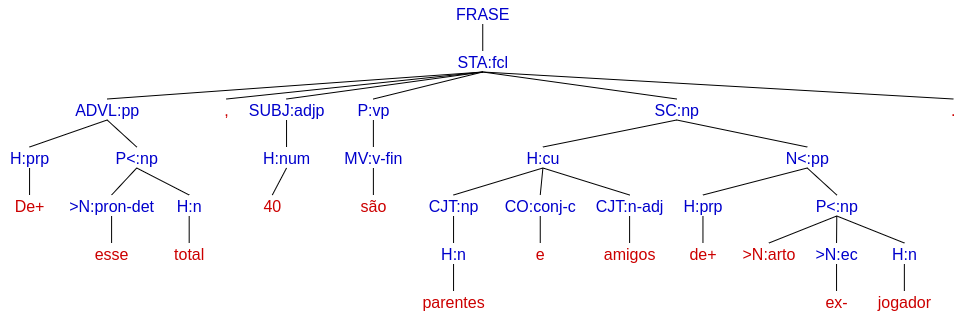
\includegraphics[width=\linewidth]{imagens/ec_bosque_ec_tree_orig.png}
        \caption{árvore original}
    % \end{subfigure}
    \end{minipage}
    % 
    \begin{minipage}{.45\textwidth}
        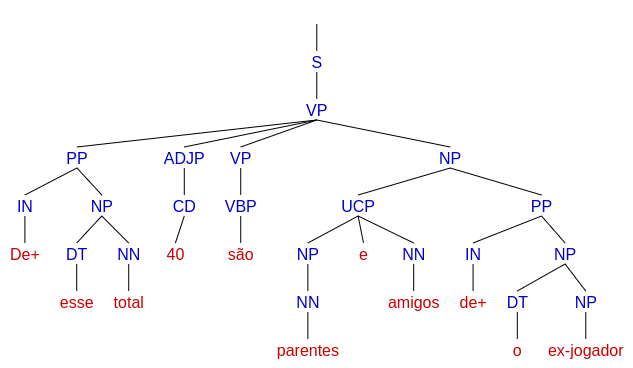
\includegraphics[width=\linewidth]{imagens/ec_bosque_ec_tree_trans.png}
        \caption{árvore transduzida}
    \end{minipage}
    \begin{minipage}{.45\textwidth}
        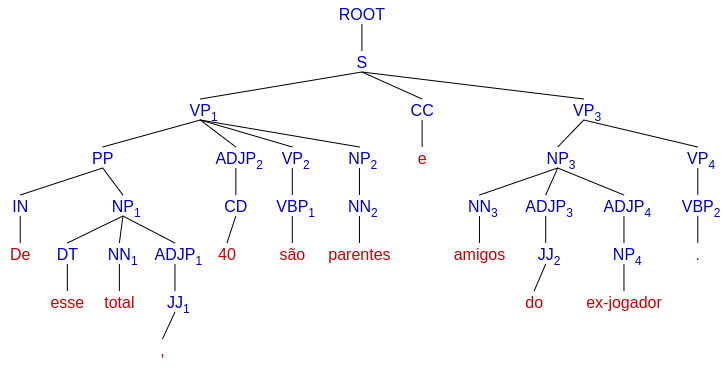
\includegraphics[width=\linewidth]{imagens/ec_bosque_ec_tree_ps.png}
        \caption{árvore gerada pelo SP}
    \end{minipage}
    % \begin{minipage}{.45\textwidth}
    %     \ldots
    %     \begin{tabbing}
    %         \=(NP\= (JJ ,) (NN Dawn)\+\\
    %         \>  (AD\=JP (JJ Upshaw)))\-\\
    %         \>(CC e)\\
    %         \>(VP\=\+\\
    %         \>  (VP (VBP Galina))\\
    %         \>  (NP\= (NN Gorchakova)\+\\
    %         \>      (ADJP (JJ .))))))))
    %     \end{tabbing}
    % \end{minipage}
    \caption[Estudo de caso BOSQUE - Sentença transduzida com \textit{ec}, e \textit{cu}]{Estudo da sentença CF866-2, \textquote{De esse total, 40 são parentes e amigos do ex-jogador.}, que possui a \textit{tag} \textit{ec}.}
    \label{fig:ec_bosque_ec_tree}
\end{figure}